%%%%%%%%%%%%%%%%%%%%%%%%%%%%%%%%%%%%%%%%%
% Structured General Purpose Assignment
% LaTeX Template
%
% This template has been downloaded from:
% http://www.latextemplates.com
%
% Original author:
% Ted Pavlic (http://www.tedpavlic.com)
%
% Note:
% The \lipsum[#] commands throughout this template generate dummy text
% to fill the template out. These commands should all be removed when 
% writing assignment content.
%
%%%%%%%%%%%%%%%%%%%%%%%%%%%%%%%%%%%%%%%%%

\documentclass{article}

\usepackage{fancyhdr} % Required for custom headers
\usepackage{lastpage} % Required to determine the last page for the footer
\usepackage{extramarks} % Required for headers and footers
\usepackage{graphicx} % Required to insert images
\usepackage[latin1]{inputenc}

% Margins
\topmargin=-0.45in
\evensidemargin=0in
\oddsidemargin=0in
\textwidth=6.5in
\textheight=9.0in
\headsep=0.25in 

\linespread{1.1} % Line spacing



\setlength\parindent{0pt} % Removes all indentation from paragraphs

%----------------------------------------------------------------------------------------
%	DOCUMENT STRUCTURE COMMANDS
%	Skip this unless you know what you're doing
%----------------------------------------------------------------------------------------

% Header and footer for when a page split occurs within a problem environment
\newcommand{\enterProblemHeader}[1]{
\nobreak\extramarks{#1}{#1 continued on next page\ldots}\nobreak
\nobreak\extramarks{#1 (continued)}{#1 continued on next page\ldots}\nobreak
}

% Header and footer for when a page split occurs between problem environments
\newcommand{\exitProblemHeader}[1]{
\nobreak\extramarks{#1 (continued)}{#1 continued on next page\ldots}\nobreak
\nobreak\extramarks{#1}{}\nobreak
}

\setcounter{secnumdepth}{0} % Removes default section numbers
\newcounter{homeworkProblemCounter} % Creates a counter to keep track of the number of problems
%----------------------------------------------------------------------------------------
%	NAME AND CLASS SECTION
%----------------------------------------------------------------------------------------

\newcommand{\lessonNumber}[1]{Lezione\ \##1} % Assignment title
\newcommand{\lessonDate}[4]{#1,\ #2\ #3\ #4} % Due date
\newcommand{\lessonCourse}[1]{#1} % Course/class
\newcommand{\lessonTime}[1]{#1} % Class/lecture time
\newcommand{\lessonTeacher}[1]{#1} % Teacher/lecturer
\newcommand{\lessonAuthor}[1]{#1} % Your name

% Set up the header and footer
\pagestyle{fancy}
\lhead{\lessonAuthor{Luca De Franceschi}} % Top left header
\chead{\lessonAuthor{Tullio Vardanega}\ \lessonTime{9:30}: \lessonNumber{16}} % Top center header
\rhead{\firstxmark} % Top right header
\lfoot{\lastxmark} % Bottom left footer
\cfoot{} % Bottom center footer
\rfoot{Page\ \thepage\ of\ \pageref{LastPage}} % Bottom right footer
\renewcommand\headrulewidth{0.4pt} % Size of the header rule
\renewcommand\footrulewidth{0.4pt} % Size of the footer rule

%----------------------------------------------------------------------------------------
%	TITLE PAGE
%----------------------------------------------------------------------------------------

\title{
\vspace{2in}
\textmd{\textbf{\lessonNumber{16}}\\
\normalsize\vspace{0.1in}\small{\lessonDate{Gioved�}{14}{Novembre}{2013}}\\
\vspace{0.1in}\large{\textit{\lessonTeacher{Tullio Vardanega},\ \lessonTime{9:30-11:30}}}
\vspace{3in}
}
}

\author{\textbf{\lessonAuthor{Luca De Franceschi}}}
\date{} % Insert date here if you want it to appear below your name

%----------------------------------------------------------------------------------------

\begin{document}

\maketitle
\newpage
\newpage

Chi compra vuole comprare da fornitori che siano qualificati e che diano una certa garanzia -> \textbf{CMM}\\
\textbf{SPICE}, iniziativa per cercare di trovare una valutazione e un'indicazione di miglioramento sulla qualit� dei processi. Intuizione che migliorando i processi si migliorano i prodotti. Il modello \textbf{SPY} dice che poso sotto ogni processo ci dev'essere un meccanismo capace di misurare come sta andando il processo rispetto a obiettivi di qualit� misurabili. Per chiunque parla di qualit� di processo � molto importante il \textbf{CMMI}:

\begin{itemize}

	\item \textbf{Capability}, capacit� di fare le cose, misurazione di quanto un processo � fatto bene e rispetta i suoi obiettivi;
	\item \textbf{Maturity}, misura qual'� la soglia pi� bassa delle capability di processo su tutti i processi che l'azienda attua. Se un'azienda � brava a fare una cosa ma non lo � a fare le altre non � una buona azienda.
	\item \textbf{Model};
	\item \textbf{Integration}, prima questa cosa era applicata al software, ora anche ad altre cose.

\end{itemize}

La sua logica � che ``non possiamo funzionare che a processi, le organizzazioni devono imparare a funzionare a processi perch� otterranno il massimo risultato. Si dice che un'organizzazione capace di effettuare miglioramenti sui processi � in grado di fare \textbf{governance}, sinonimo di efficacia, efficienza, mantenibilit� e visione. Gestire la qualit� di processi non sta al Project Manager ma ad uno strato pi� importante che sta sopra e ha una visione pi� ampia e possiede una strategia di lungo periodo riferita al miglioramento. Molte aziende hanno \textit{management} ma non hanno \textit{governance} e ad un certo punto si estinguono perch� non hanno la capacit� di adattarsi ai cambiamenti. Il \textbf{CMM} ha il concetto di \textbf{scala}.

\begin{center}
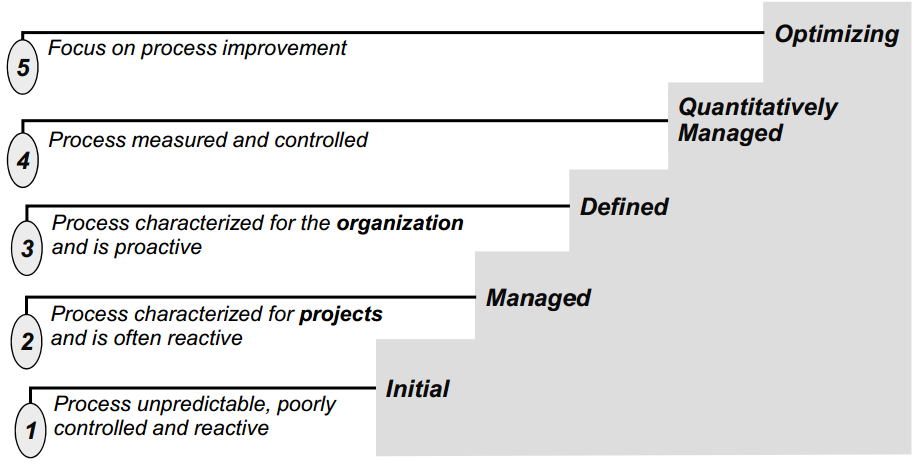
\includegraphics[width=0.75\columnwidth]{img1.png} % Example image
\end{center}

Si parte da osservare che al piano terra c'� uno strato iniziale in cui tutti all'inizio si collocano. I processi, se ci sono, sono a questo stadio \textbf{unpredictable}, impredicibili, \textbf{poorly controlled} e \textbf{reacted}. Il livello 2 � \textbf{managed}, cio� gestito. I processi esistono nei progetti e rimangono prevalentemente reattivi. Il livello 3 � \textbf{definito}, i processi sono proattivi, esistono trasversalmente, manca ancora il miglioramento. Il livello 4 introduce misurazione rispetto al controllo e si chiama \textbf{quantitatively managed}. Al livello 5 non soltanto misuriamo ma miglioriamo, \textbf{optimizing}. Dove un'azienda si colloca in questa scala dipende fortemente dalla domanda che c'� in un preciso ecosistema (paese).\\
Riflettere su come mi organizzo per effettuare un determinato processo. Adottando il CMMI aumento del 35\% la produttivit�, riduco del 19\% il \textbf{time to market} e riduco del 39\% il \textbf{post-release defect reports} (proporzione di difetti residui, ovvero costi di manutenzione).\\
ISO/IEC 15504-2 � un documento simile a CMM che disarticola ogni processo in caratteristiche rilevanti su quel processo e su ogni attributo di processo attacca un'etichetta che dice a che punto siamo su quel processo.\\
Capito questo bisogna concentrarsi su come lavoriamo, imparare i processi e cercare di migliorarli. Fare lo sforzo di funzionare a processi non � abbastanza, siamo al livello 3, vogliamo almeno andare al 4.

\end{document}